% !TEX TS-program = xelatex
% !TEX encoding = UTF-8 Unicode
% !Mode:: "TeX:UTF-8"

\documentclass{resume}
\usepackage{zh_CN-Adobefonts_external} % Simplified Chinese Support using external fonts (./fonts/zh_CN-Adobe/)
%\usepackage{zh_CN-Adobefonts_internal} % Simplified Chinese Support using system fonts
\usepackage{linespacing_fix} % disable extra space before next section
\usepackage{cite}
\usepackage{tabu}
\usepackage{multirow}
\usepackage{adjustbox}
\hypersetup{
hidelinks,
colorlinks=true,
linkcolor=purple,
citecolor=purple
}

% Tighter page and section spacing so the whole résumé stays on one page.
\geometry{left=0.75in, right=0.75in, top=0.55in, bottom=0.4in}
\titlespacing*{\section}{0cm}{*1.0}{*0.8}
\titlespacing*{\subsection}{0cm}{*1.1}{*0.4}
\begin{document}
\pagenumbering{gobble} % suppress displaying page number

\begin{minipage}[c]{0.82\textwidth}
\name{刘祎铭}
{\centering\sffamily\large
  \email{letusgo126@gmail.com} \textperiodcentered\
  \phone{(+86) 130-0927-5407}\\[0.4ex]
  \github[github.com/LYMDLUT]{https://github.com/LYMDLUT} \textperiodcentered\
  \homepage[lymdlut.github.io]{https://lymdlut.github.io/}
  \par}
\vspace{1.5ex}
\end{minipage}%
\begin{minipage}[c]{0.18\textwidth}
\raggedleft
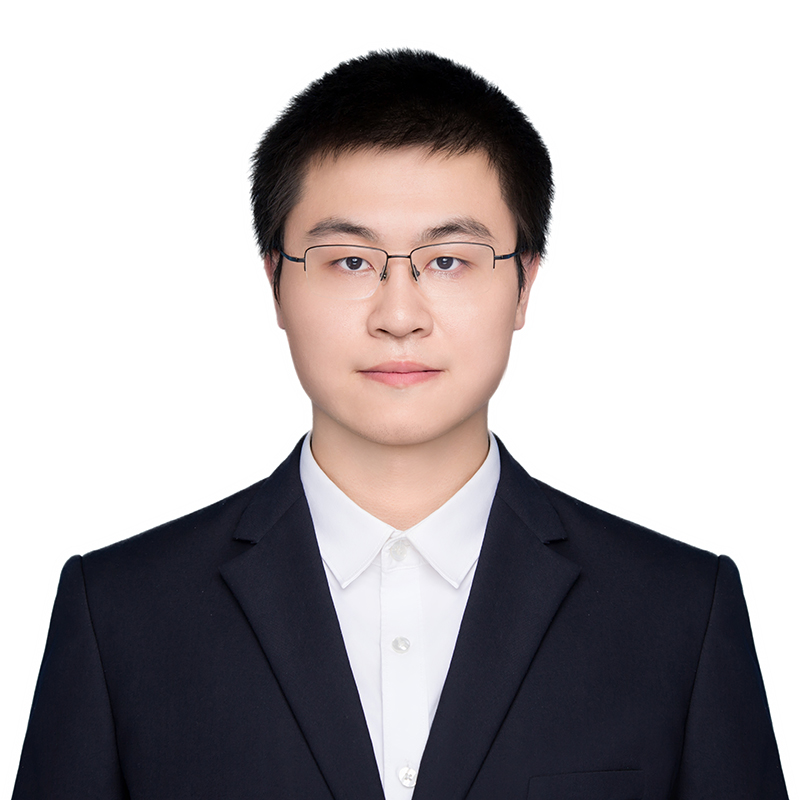
\includegraphics[width=0.88in]{photo.jpg}
\end{minipage}

\section{\faGraduationCap\  教育背景}
\datedsubsection{\textbf{中山大学}, 广州}{2022 -- 2025}
\textit{硕士研究生}\ 计算机视觉\\
\href{https://www.sysu-hcp.net}{人机物智能融合实验室 (HCP Lab)}，导师为林倞教授\textit{(杰青，IEEE Fellow)}
\vspace{-0.3cm}
\datedsubsection{\textbf{大连理工大学}, 大连}{2018 -- 2022}
\textit{学士}\ 电子信息工程\quad
GPA : 4.59/5, 排名 \textcolor{red}{4}/206

\section{\faUsers\ 工作与研究经历}

\datedsubsection{\textbf{大模型评测 (腾讯混元)}}{2025年7月 -- 至今}
\begin{itemize}
  \item \textbf{评测基准}：构建 \href{https://arxiv.org/abs/2605.26380}{\textbf{VisualNeedle}}（信息密集场景下的主动视觉搜索，提出 crop-black 反事实设置，因果验证模型是否真正使用了工具返回的视觉证据）、\href{https://hanxiao.io/jy-crpg-bench/}{\textbf{jy-crpg-bench}}（开放世界 RPG 中的长程任务）、\href{https://arxiv.org/abs/2601.01400}{\textbf{EternalMath}}（随人类新发现生长的数学基准）等评测基准
  \item \textbf{图文一致性评估}：构建 Agent 流水线，通过绘图指令拆解、构造问答对、LLM 综合打分评估图文一致程度，并自动归因到出错的类别/元素；在模型排序和未对齐元素判定上与人工高度一致，已优化时间与金钱成本并部署落地
  \item \textbf{视频打分模型训练}：将视频质量拆分为图文一致、视觉质量、动态质量三个维度，自建 1w 内部数据集，探索 SFT、RL、冻结打分在 VLM 上的应用，在自建和公开 bench 上均达到 SOTA，总结为技术报告 \href{https://arxiv.org/abs/2511.18825}{\textbf{Q-Save}}
\end{itemize}

\datedsubsection{\textbf{OpenRLHF 强化对齐算法与框架开发}}{2024年9月 -- 至今}
\begin{itemize}
  \item \textbf{框架}：主导 \href{https://github.com/OpenRLHF/OpenRLHF}{OpenRLHF} 中 KL 损失算法，以及 DeepSpeed AutoTP、FSDP2+CP+TP 等训练后端开发
  \item \textbf{算法}：首次发现 GRPO 中 k3 loss 作为损失函数的有偏性，提出无偏的 k2 loss，博客被 \href{https://arxiv.org/abs/2501.03262}{Reinforce++} 引用，并总结为技术报告 \href{https://arxiv.org/abs/2510.01555}{\textbf{Rethinking KL Regularization in RLHF}}
\end{itemize}

\datedsubsection{\textbf{基于扩散模型的对抗净化防御算法 (中山大学 HCP Lab)}}{2023年3月 -- 2025年4月}
\begin{itemize}
  \item \textbf{分析}：提出新的解释角度，认为 Diffusion 的对抗防御能力来源于随机性、且其 Loss landscape 局部并不平坦，而非既有研究中的“前向加噪减小自然图片与对抗图片的 KL 散度”或“高斯噪声的掩盖效应”，并首次将其与 Certified robustness 中的随机性区分开
  \item \textbf{方法}：提出扩散去噪对抗训练算法，通过平滑 Loss landscape 增强防御能力，在 DDPM、DDIM、VP-SDE、EDM 等扩散模型和多个数据集上一致提升
\end{itemize}

\datedsubsection{\textbf{MMDetection 算法框架开发 (上海 AI Lab)}}{2022年7月 -- 2023年3月}
Detection Transformer 系列算法在 MMDetection 2.0 和 3.0 两个大版本深度重构与新增复现的核心成员
\begin{itemize}
  \item 简化注册机制与继承关系，统一模块数据格式，大幅提升代码可读性、可维护性与运行效率，MMDetection 专门为本次工作新增 GitHub 分支 \href{https://github.com/open-mmlab/mmdetection/tree/refactor-detr}{refactor-detr}
  \item 复现重构 Conditional/DAB DETR、DINO 等复杂算法，统一混乱的模块命名与抽象逻辑，严格对齐性能指标并补充文档注释；受邀在 \href{https://www.bilibili.com/video/BV17x4y1w7ZK/?spm_id_from=333.337.search-card.all.click}{OpenMMLab 社区开放麦}讲解本次工作
\end{itemize}

\section{\faPrint\ 论文}
{\small
\begin{itemize}
  \item \textbf{ICLR 2025}\quad \textit{(第一作者)} Towards Understanding the Robustness of Diffusion-Based Purification: A Stochastic Perspective
  \item \textbf{EMNLP 2025 Demo}\quad OpenRLHF: A Ray-based Easy-to-use, Scalable and High-performance RLHF Framework
  \item \textbf{投稿中}\quad \textit{(第二作者)} jy-crpg-bench: A Long-Horizon Benchmark for Frontier Models in an Open-World RPG
  \item \textbf{投稿中}\quad \textit{(共同一作)} VisualNeedle: Benchmarking Active Visual Search in Information-Dense Scenes
  \item \textbf{arXiv}\quad Rethinking KL Regularization in RLHF: From Value Estimation to Gradient Optimization
  \item \textbf{arXiv}\quad Q-Save: Towards Scoring and Attribution for Generated Video Evaluation
  \item \textbf{arXiv}\quad EternalMath: A Living Benchmark of Frontier Mathematics that Evolves with Human Discovery
  \item \textbf{arXiv}\quad DramaChain Bench: An End-to-End Benchmark for Short-Drama Generation
\end{itemize}
\par}

\section{\faCogs\ 专业技能}
\begin{itemize}
  \item 关注方向：大模型评测（基准设计、自动打分与归因）、RLHF/RLVR、Agent RL
  \item 并行与训练：基于 DTensor 的 FSDP2 系列并行、DeepSpeed、Ray + vLLM 的 RLHF 训练链路
\end{itemize}

\end{document}
